\documentclass[conference]{IEEEtran}

\usepackage{url}
\usepackage{graphicx}

\hyphenation{op-tical net-works semi-conduc-tor}

% Document.
\begin{document}

\title{Comparative Analysis of Performance Using Server-Client Protocols}

\author{\IEEEauthorblockN{Mihail Costea}
\IEEEauthorblockA{University Politehnica of Bucharest\\
The Faculty of Automatic Control and Computers\\
Bucharest, Romania\\
Email: mihail.costea90@gmail.com}
\and
\IEEEauthorblockN{Liviu Chircu}
\IEEEauthorblockA{University Politehnica of Bucharest\\
The Faculty of Automatic Control and Computers\\
Bucharest, Romania\\
Email: liviu.chircu@gmail.com}}

\maketitle

\begin{abstract}
Current web applications' solutions for bi-directional communication are widely
based on AJAX. Even though they are well documented solutions that are backed up by
years of utilization, they have limitations imposed by the HTTP protocol. HTTP
is a stateless protocol that requires each connection to be treated as a new
connection, requiring an unnecessary overhead to communicate in both directions.
Because of these limitations, a new solution was developed - WebSockets -
which are able to natively mantain a bi-directional channel, thus reducing the
overhead imposed by connection establishment.
\\
\indent
This paper proposes to exemplify the advantages and disadvantages between
traditional HTTP implementations for bi-directional communication based on AJAX
and WebSockets. It also proposes an architecture for a testing platform for
different WebSockets implementations.
\end{abstract}

\IEEEpeerreviewmaketitle

% Content.
\section{Introduction}
Along with the introduction of Web 2.0, web applications have been able to
modify the content of HTML documents without the need of a complete page
refresh, offering a more interactive environment for the end-user.
The most popular technology used to create this interactivity is AJAX \cite{AJAX}
(Asynchronous JavaScript and XML). With AJAX, pages can be updated in real-time,
without needing an explicit action from the user. But because AJAX is based on
HTTP - a stateless protocol that requires each connection to be treated as a new
connection - bi-directional channels between 2 devices can only be simulated
through a series of methods which impose a significant amount of overhead, as both
nodes need to mimic this channel that require states.
Bi-directional channels are necessary for web applications such as instant
messaging clients, browser-based games, video calls, etc., where large amounts
of traffic (with complete sets of headers and message bodies) need to be sent from
each endpoint over to the opposite one.
\\
\indent
The most popular solutions used by AJAX are: \textbf{polling}, where a client sends
a request to a server at regular intervals with the server responding immediately
and closing the connection; \textbf{long-polling}, where the client requests
information from the server just as in normal polling, but the server now maintains
its connection open until it has the data to send, point in time where
it will send an immediate response;
\textbf{streaming}, where the connection between the client and the server is
kept alive indefinitely and data is streamed until one of the two closes the
connection. The problem with last solution is that AJAX
appends the new data to previously sent data until the connection ends, which is
unnecessary in many cases. Moreover, HTTP headers must be sent whenever a new
connection is created, which is a common case for polling and long-polling. If
a great amount of small pieces of data are to be sent, as in the case of a
web-based chat application, the overhead of the headers might actually overweigh
the data that is actually transmitted \cite{2009:Misc}.
\\
\indent
In order to overcome the limitations of AJAX-based solutions, the HTTP-based
WebSockets protocol was created \cite{RFC}. HTTP was chosen as a base because
most firewalls allow HTTP and HTTPS traffic  (ports 80 and 443), while other
ports' traffic might be blocked. Although based on HTTP, WebSockets do not
inherit its limitations. HTTP is only used to create and close the connection
between client and server, while the in-between information exchage is done
through a series of WebSocket-specific data frames. The distinction between
normal HTTP traffic and WebSockets is done through the "Upgrade: websocket" /
"Connection: Upgrade" headers \cite{RFC}.
\\
\indent
As mentioned above, WebSockets are a recently created technology 
(the RFC was written in 2011), so they are not supported by all major
web servers, let alone being extensively tested. This may
very well be considered a downside when compared to AJAX, which benefits from
years of testing and industry usage. Although a series of testing platforms
with the purpose of validating WebSockets implementations have been created,
like Autobahn \cite{Autobahn}, to our best knowledge, we have yet to find any
performance-oriented testing platforms for a given WebSockets implementation.
This paper compares AJAX with WebSockets and proposes an architecture for
a testing platform, which should be independent of the underlying Operating
System and present devices. It should work for both laptops and smartphones,
for Windows and Linux and other devices and Operating Systems.

\section{Related work}
\textit{Real-time Monitoring using AJAX and WebSockets} \cite{RT-Monitoring}
exemplifies the differences in terms of performance between AJAX and WebSockets.
The authors added real-time monitoring support for OASIS \cite{OASIS},
an open-source real-time instrumentation middleware for distributed real-time
and embedded systems. The collected instrumentation data was sent over the Web
using AJAX and WebSockets and the results were compared. The WebSockets server
consumes 50\% less network bandwidth than the AJAX server. Also, the WebSockets
client consumes memory at a constant rate, while the AJAX client consumes it
at an increasing rate. Furthermore, the WebSockets-oriented implementation can
send up to 215.44\% more data samples than the AJAX-based counterpart although
demanding the same amount of network bandwidth.
\\
\begin{frame}{}
  \begin{figure}
    \centering
    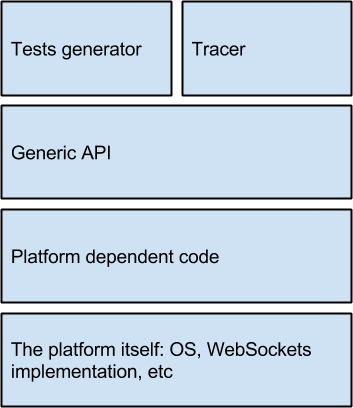
\includegraphics[width=0.4\textwidth]{Architecture.png}
    \caption{Performance application architecture}
  \end{figure}
\end{frame}
\indent
Another example where WebSockets are better than AJAX is the case of sending
small data per frame. While WebSockets exchange 2B of data per frame, continuous
polling with AJAX exchange up to 8 KB of HTTP header \cite{2009:Misc}.
\\
\indent
Even though WebSockets are better than AJAX based solutions, it's still not as
good as raw TCP sockets. \textit{Real-time Web Application Roadblock:
Performance Penalty of HTML Sockets} paper \cite{Performance-Penalty} discusses
the penalties of using HTML socket streams (long-polling and WebSockets)
versus TCP streams. HTML socket streams can have up to 5x protocol overhead, up to
3x more payload delivery delay and up to 3x less throughput. In case of small
data payload (a few hundreds of bytes), the performance between the two becomes
significantly noticeable. Also TCP streams tend to behave better over 3G than
HTML socket streams.
One reason for the poorer performance is due to the fact that the browser uses
buffering for HTML socket streams (both long-polling and WebSockets), thus 
introducing delays, while TCP sockets are able to send the data directly.
But on the good side for
WebSockets, the paper mentions that they behave better than long-polling when
it comes to sending small-sized chunks, making it a better choice for chat,
VoIP, online games, etc, just like TCP streams. A big plus for HTML sockets
over TCP streams is the fact that the data sent through them can pass over
firewalls and most proxies, as HTTP and HTTPS are commonly allowed ports.

\section{Evaluating existing WebSocket implementations}
In order to get a better idea about how different WebSockets implementations
behave and how the architecture of the testing application should be designed, a
series of tests were performed on two different Node.js WebSocket implementations.

The chosen implementations are \textbf{ws} \cite{nodejs-ws}
and \textbf{WebSocket-Node} \cite{nodejs-websocket}, both part of Node.js
\cite{nodejs}. The tests were performed on an Intel Core i7-4770 with 16GB of
RAM running on Ubuntu 13.10, 64-bit. As a measuring tool we have used the
\textit{Look} performance profiler for Node.js \cite{nodejs-look}, which offered
information about the process's CPU time, RSS (Resident Set Size), V8 heap total
\cite{javascript-v8}, V8 heap used, and OS load average.
\indent
We have tested 4 different scenarios:

1. Connected 4 clients simultaneously every second until 3400 connections were reached.
All connections are kept alive during the entire run and transferred data is negligible
(a single number). Figure X (TODO) contains the comparison between the two WebSockets
implementations. We can observe that \textbf{ws} has a better CPU usage when handling
fewer connections than \textbf{WebSocket-Node}, but towards the end they behave almost
similar. The memory consumption of the two is also similar.

2. Connected 600 clients simultaneously once every 120 seconds. All connections are
kept alive during the entire run and transferred data is negligible (a single number).
Figure X (TODO) contains the comparison between the two websockets implementations.
Following the conclusions of the first example, memory consumption is similar and
\textbf{ws} is faster than \textbf{WebSocket-Node}, but under extremely heavy weight,
the system freezes faster for \textbf{ws}. We were able to go only up to 3600 connections
with \textbf{ws}, while \textbf{WebSocket-Node} peaked at 4200 connections.

3. Simultaneously connected 100 clients right away, which exchanged data with
sizes ranging from 2KB up to 1MB, with increments of 2KB/s per client. All
connections were kept alive during the entire run, and no extra clients were
added. Clients simply send more data with every second. Figure X (TODO)
contains the comparison between the two WebSockets implementations. In this
example we can clearly see that \textbf{WebSocket-Node} behaves better when
sending large packets. At almost 1MB / packet, \textbf{WebSocket-Node}
processes everything in under 2s, but \textbf{ws} requires up to 6s. Also
we had to stop \textbf{ws} before 1MB / packet because the system almost freezed,
while the other implementation allowed us to let it reach its limit.

4. Simultaneously connected 400 clients, then closed their connections after 10
seconds. Once every 90 seconds, 200 clients would be added to the prior number
of clients, and the first steps would be repeated.
The process continued until 2800 connections
were reached. Transferred data was negligible (a single number). Figure X (TODO)
contains the comparison between the two websockets implementations. In this
example the used memory is similar, but the \textbf{ws} implementation has
bigger peaks for CPU usage than \textbf{WebSocket-Node} when it comes to the
last few iterations, where large numbers of connections must be managed
(more than 2200). For small numbers of connections, both implementations behave
similar.

% FIXME: Conclusions subtitle?
We arrived at the conclusion that \textbf{ws} is faster than
\textbf{WebSocket-Node} when it comes to fewer connections and small data
packets, but with larger-sized packets and sizeable amounts of connections,
\textbf{WebSocket-Node} seems to behave better.


\section{Architecture}
This section proposes a simple architecture for an application which is capable
of testing the performance of WebSockets and AJAX implementations of bi-directional
communication. Figure 1 contains the architecture and the layers. In order to
test the performance automatically, the application should be able to generate
tests based on a given input and automatically measure how those tests behave
on a given platform. The design should promote easy porting to other devices
and Operating Systems. It should have a layer which is independent of 
platform and implementation (either WebSockets or AJAX). The layer provides a generic
API that is used by the tests generator component and the tracer or measurements
component. The API and the previously mentioned components are going to be ported
to other platforms with minimal changes. The layer that provides the API is going
to be implemented by every platform in a different way, depending on the
Operating System, specific WebSockets API requirements, etc.

\bibliography{bare_conf}{}
\bibliographystyle{unsrt}

\end{document}


